\documentclass{article}


\title{Hashing and Bloom filters key lookup comparison}
\author{names}
\date{\today}

\usepackage{lipsum}
\usepackage[backend=bibtex]{biblatex}
\usepackage{graphicx}
\usepackage{amsmath}

\bibliography{references}
\nocite{*}

\begin{document}
    \maketitle
    \thispagestyle{empty}
    \begin{abstract}
        \lipsum[1]
    \end{abstract}


    \section{Introduction}
        \lipsum[2]

    \section{Experiment pipeline and methodology}
        \lipsum[1]
	\begin{figure}
	  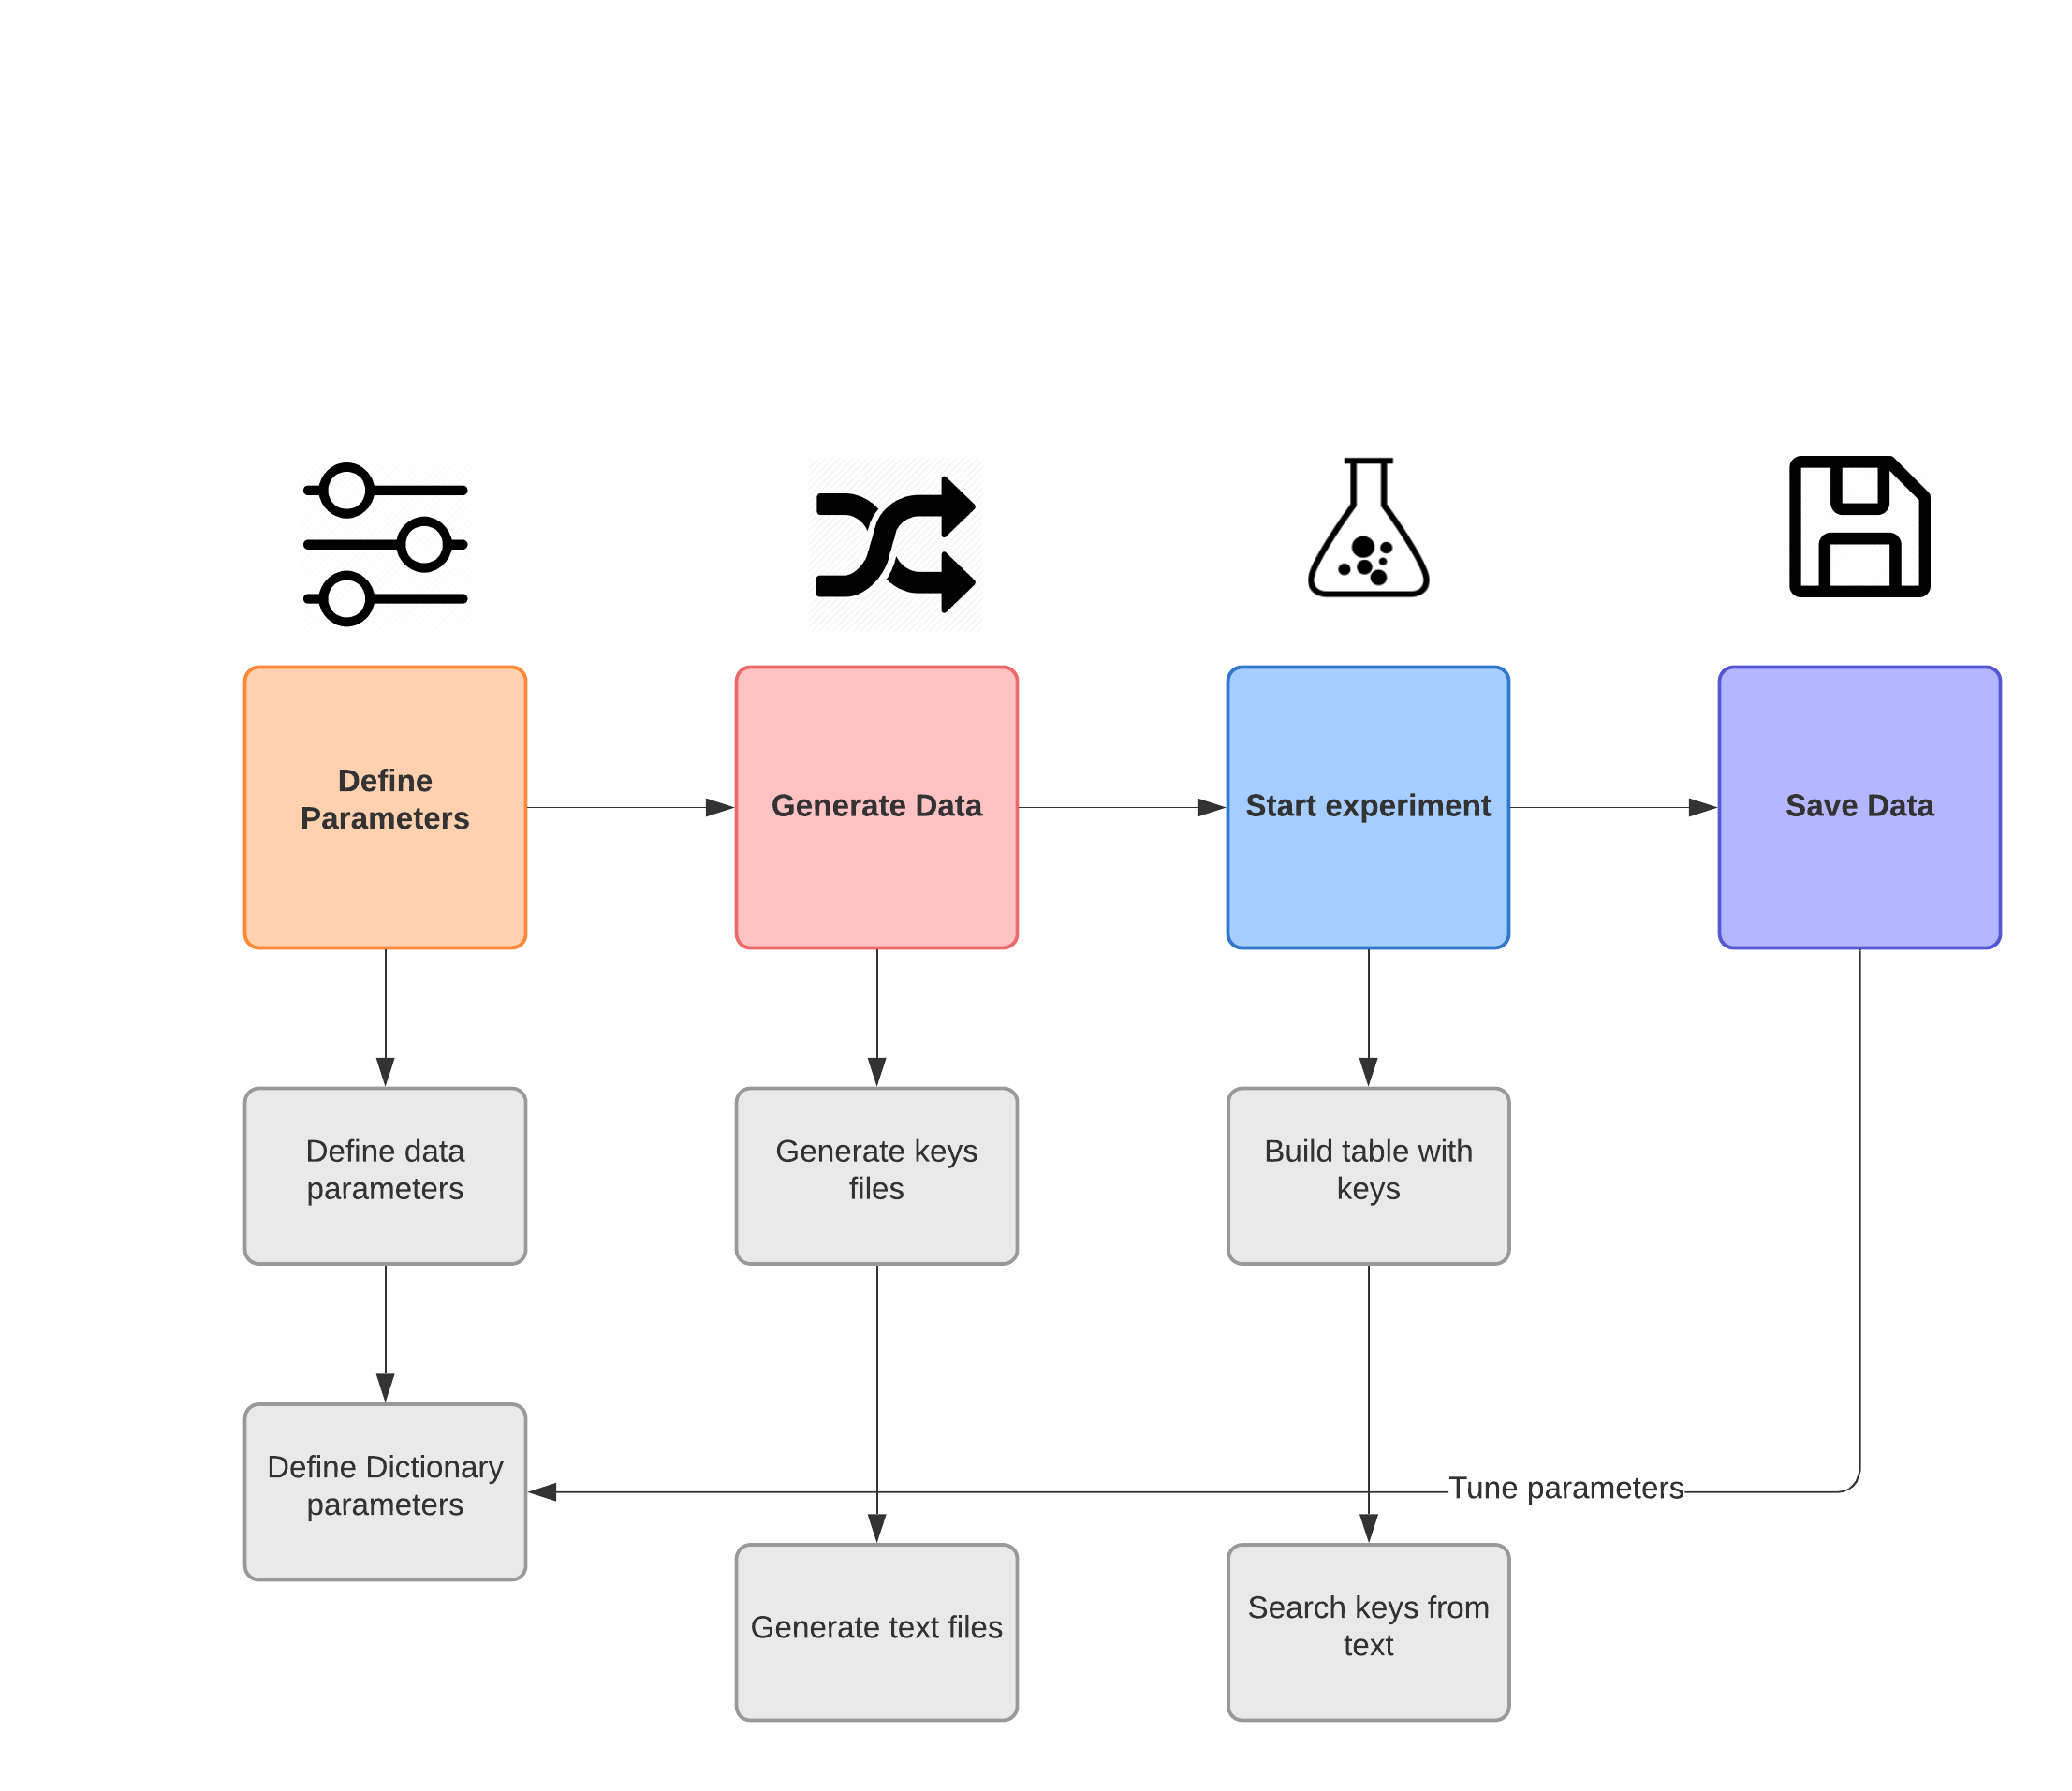
\includegraphics[width=\linewidth]{experiment_pipeline.png}
	  \caption{Experiment pipeline}
	  \label{fig:Pipeline}
	\end{figure}
	\lipsum[1]
    \section{Data Generation}
        The data used in each of the experiments consisted of a sequence of unsigned integers,  the data was written in two different files, to distinguish them we used a specific format specified in figure X. One file contained the keys to insert into the dictionary and the other the text to find in the dictionary. The keys file contained n numbers and the text contained $2 * n + p * n$ where $p$ is the percentage of keys that are already inserted in the dictionary.
		\begin{center}		
		\begin{figure}[h]
	  		
\includegraphics[scale=0.25]{data_file_format.png}
	  		\caption{Data file format}
	  		\label{fig:File format}
		\end{figure}
		\end{center}
		\subsection*{Linear Congruential Method}
		The randomness of the keys was based on the Linear congruential method (LCM). We needed to have experiments as reliable as possible thus we needed a way to control the data generation, that is why we used this method. The LCM is one of the oldest and best-known random number generators, it is also very easy to implement. This method generates a cyclic sequence of numbers based on an initial seed. Given a seed $X_0$ it is possible to generate the next number in the sequence $X_i = (X_{i-1} * a + c)$ $mod$ $m$, where $a$ is called the multiplier, $c$ the incrementer and $m$ the modulus. The size of the sequence depends on the parameters used, independently on the initial seed. The best parameters are the ones that yield the maximum size sequence, that is parameters that yield $m$ numbers, to get this performance we need to ..... ETC.  The parameters that we used where ...
    \section{Experiment parameters}
        \lipsum[1]
    \section{Results}

    \section{Discussion}
        \lipsum[1]


    \printbibliography

\end{document}
